    \begin{figure}[H]
    	
\includegraphics[scale=0.40]{pictures/logo2.png}
    \end{figure}

\section{About}
    Game concept is a detailed description of the game, including information such as high concept, genre,
    gameplay description, features, setting, story, target audience, hardware platforms, estimated schedule,
    marketing analysis, team requirements and risk analysis. Source: 
    \url{en.wikipedia.org/wiki/Game_development#Development_process}
    Several of these points like the risk analysis and hardware platforms have been brought up in other 
    sections of the report and will not be discussed here. This section will mainly be about the gameplay. 
    The game concept is the basis for the game's functional requirement. It is easier to explain the game 
    as well as decide on the functional equirements for the game on the basis of the game concept. 


\section{High Concept}
    The name for the game we settled on is Power Supply. It is in the construction and management 
    simulation genre and is inspired by games like SimCity, only in a more limited scope. You are 
    tasked with managing the delivery of electricity to cities and factories in an area, while the 
    ultimate goal of the game is making money as the tycoon of the local power company, without going 
    bankrupt.

\section{Gameplay Description}

\subsection*{Player}
    The role of the player is to build powerplants to supply the buildings on the game map with power. 
    To do this the player has to connect the powerplants to the buildings with powerlines. Either directly
    or indirectly. Building powerplants and powerlines costs money. To earn money the player has to supply
    power to the buildings on the map. If the inhabitants of a building does not get power then they will
    move out and abandon the building. If too many buildings become abandoned then the game is over.
    Abandoned buildings disappear from the game.

\subsection*{Powerplants}
    Powerplants can only supply a fixed amount of power to the connected buildings. If a powerplant is 
    unable to supply power to all the buildings on the map, the player has three options. The first option 
    is to build more powerplants. The second powerplant can then be connected to the buildings that the
    player wasn't previously able to supply with power. The second option is to upgrade the powerplant,
    so that it can deliver more power. This is supposed to be more cost effective in the short term, however
    it can become more expensive in the long run because of other important factors which will be brought
    up later. The final option is to demolish an already existing powerline and allow the powerplant to
    supply another building with power. This could be risky, as buildings that are not supplied with power
    will eventually become abandoned.

\subsection*{Powerlines}
    Powerlines is the way the player connects their powerplants to the buildings in need of power. This 
    can be done directly or indirectly. A direct connection is a connection between a powerplant and a 
    building in need of power. While an indirect connection is to connect a building with another building.
    Power from the powerplant then travels through the directly connected powerlines and continues down 
    the indirectly connected powerlines, supplying as many buildings as possible with power. Direct 
    connections are important, since buildings that are directly connected will receive power first.
    However you also have to consider the length of the powerline, as longer powerlines are more expensive
    to build than short powerlines. You can also tear down powerlines in order to supply other buildings
    with power.

    \begin{figure}[!ht]
    \centering
    \subfigure{
      
\includegraphics[scale=1]{pictures/coin.png}
    }
    \subfigure{
      
\includegraphics[scale=0.45]{pictures/factory_1_128.png}
    }
    \subfigure{
      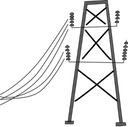
\includegraphics[scale=0.45]{pictures/pylon.png}
    }
    \caption{Game Elements}
    \end{figure}


\subsection*{Buildings}
    In the game, buildings is are appearing randomly at random positions. The buildings are different
    because in the real world, the bigger the house, then the house require more power. There is 6 kind
    of buildings that will appear on the map. 


    \begin{figure}[!ht]
    \centering

    \subfigure{
      
\includegraphics[scale=0.45]{pictures/house_2_128.png}
    }
    \subfigure{
      
\includegraphics[scale=0.45]{pictures/house_1_128.png}
    }
    \subfigure{
      
\includegraphics[scale=0.45]{pictures/house_3_128.png}
    }
    \subfigure{
      
\includegraphics[scale=0.45]{pictures/house_4_128.png}
    }
    \subfigure{
      
\includegraphics[scale=0.45]{pictures/factory_2_128.png}
    }
    \subfigure{
      
\includegraphics[scale=0.45]{pictures/company_1_128.png}
    }
    \caption{The buildings in the game}
    \end{figure}

\subsection*{Goal}
    When you start a new game you will always get a goal. The goal is how money you need to
    reach in order to go to the next level. 
